%%%%%%%%%%%%%%%%%%%%%%%%%%%%%%%%%%%%%%%%%%%%%%%%%%%%%%%%%%%%%%%%%%%%%%
% How to use writeLaTeX: 
%
% You edit the source code here on the left, and the preview on the
% right shows you the result within a few seconds.
%
% Bookmark this page and share the URL with your co-authors. They can
% edit at the same time!
%
% You can upload figures, bibliographies, custom classes and
% styles using the files menu.
%
%%%%%%%%%%%%%%%%%%%%%%%%%%%%%%%%%%%%%%%%%%%%%%%%%%%%%%%%%%%%%%%%%%%%%%

\documentclass[12pt,a4paper]{report}

\usepackage[utf8]{inputenc}
\usepackage[T1]{fontenc}
\usepackage{lmodern}
\usepackage{graphicx}
\usepackage{listings}
\usepackage{url}
\usepackage{cite}
\usepackage[top=3cm,bottom=2cm,left=3cm,right=2cm]{geometry}
\usepackage{setspace}
\usepackage{titlesec}
\usepackage{float}

% Configuração dos títulos
\titleformat{\chapter}[display]
{\normalfont\huge\bfseries}{\chaptertitle}{20pt}{\Huge}
\titlespacing*{\chapter}{0pt}{-50pt}{40pt}

\begin{document}

\begin{titlepage}
\begin{center}
    \vspace*{2cm}
    {\Huge\textbf{Implementação do Algoritmo \textit{Link State}\\em Redes de Computadores}}
    
    \vspace{2cm}
    {\Large Relatório Técnico}
    
    \vspace{4cm}
    {\Large Daniel Rodrigues de Sousa}
    
    \vspace{1cm}
    {\large Universidade Federal do Piauí\\
    Campus Senador Helvídio Nunes de Barros}
    
    \vfill
    {\large Picos - PI\\
    2024}
\end{center}
\end{titlepage}

\chapter{Introdução}

Em redes de computadores, o roteamento baseado no estado de enlace (\textit{link-state}) é uma abordagem na qual cada nó constrói uma visão completa da topologia da rede com base em informações trocadas entre vizinhos. Essa visão global permite o cálculo de rotas otimizadas utilizando algoritmos como o de Dijkstra. Diferente dos protocolos por vetor de distância, que mantêm apenas dados locais, os protocolos \textit{link-state} propagam informações sobre o estado dos enlaces por toda a rede, garantindo maior precisão e rápida convergência diante de alterações topológicas.

Nas redes móveis ad hoc (MANETs), essa abordagem enfrenta desafios significativos devido à alta mobilidade e instabilidade dos enlaces. A proposta de \cite{chen2004demand} introduz um protocolo de roteamento sob demanda, multi-caminho e baseado em estado de enlace, desenvolvido para atender aos requisitos de Qualidade de Serviço (QoS) mesmo em contextos dinâmicos. A técnica permite a manutenção de múltiplas rotas viáveis e a rápida adaptação a mudanças na topologia da rede, aumentando a confiabilidade na transmissão de dados.

Além disso, a modelagem estocástica de carga dinâmica de rede, como proposta por \cite{osorio2011dynamic}, contribui para uma avaliação mais realista do desempenho de protocolos \textit{link-state}. O modelo permite derivar distribuições probabilísticas do estado dos enlaces, reconhecendo a variabilidade do tráfego em cenários reais. Complementarmente, o estudo de \cite{park1998performance} compara o algoritmo TORA com um modelo ideal \textit{link-state}, revelando diferenças de desempenho, consumo de recursos e tempo de convergência entre as abordagens.

Neste trabalho, é apresentado um estudo aprofundado sobre a implementação e análise do algoritmo de roteamento \textit{link-state}, com ênfase em sua aplicação em redes de média escala. A implementação foi baseada no protocolo \textit{Open Shortest Path First} (\textit{OSPF}), possibilitando a simulação realista do comportamento de roteadores em um ambiente dinâmico. O simulador, desenvolvido em Python com bibliotecas especializadas, permitiu avaliar métricas como tempo de convergência, eficiência das rotas e sobrecarga de controle. Os resultados obtidos demonstram a viabilidade da proposta e sua eficácia na adaptação a mudanças topológicas, contribuindo para a compreensão prática dos mecanismos de roteamento modernos.

\chapter{Metodologia}

Este trabalho foi conduzido com base em uma abordagem sistemática para a implementação e análise do algoritmo \textit{Link State} em redes computacionais. A metodologia foi cuidadosamente estruturada para garantir consistência nos resultados, contemplando desde a configuração do ambiente de desenvolvimento até a definição das métricas de avaliação utilizadas na análise de desempenho.

\section{Ambiente de Desenvolvimento}

A implementação foi realizada utilizando a linguagem de programação Python, na versão 3.8, escolhida pela sua clareza sintática e pela ampla gama de bibliotecas voltadas ao tratamento de grafos e análise de redes. Dentre essas bibliotecas, destaca-se o uso do \textit{NetworkX} para a modelagem e manipulação da topologia de rede, bem como do \textit{Matplotlib} para a geração de visualizações gráficas que auxiliam na interpretação dos resultados. O desenvolvimento seguiu o paradigma de programação orientada a objetos, promovendo a modularização e a reutilização do código. Para garantir a consistência das dependências e a reprodutibilidade dos experimentos, foi configurado um ambiente virtual Python (\textit{venv}), no qual todas as bibliotecas necessárias foram instaladas de forma controlada.

\section{Arquitetura da Rede}

O projeto foi estruturado de forma modular, organizando os componentes em diretórios específicos que refletem suas responsabilidades. No diretório raiz \textit{link\_state\_network}, encontram-se os subdiretórios principais: \textit{docker} para os arquivos de configuração e execução dos contêineres, \textit{generate\_compose} para os geradores de topologia, e \textit{docs} para a documentação do projeto. O diretório \textit{docker} é subdividido em \textit{router} e \textit{host}, cada um contendo seus respectivos arquivos de configuração e classes de implementação. No diretório \textit{router}, a pasta \textit{class\_net} agrupa as classes principais do sistema: \textit{LSAManager} para gerenciamento de anúncios de estado de enlace, \textit{VizinhosManager} para monitoramento de vizinhos, \textit{GerenciadorDeRotas} para cálculo de rotas, e \textit{AtualizadorDeRotas} para atualização das tabelas de roteamento. A pasta \textit{test} contém os scripts de teste para verificação de conectividade, análise de rotas e visualização de topologia. O diretório \textit{generate\_compose} contém os arquivos necessários para geração dinâmica das diferentes topologias de rede suportadas (anel, estrela, árvore e linha), incluindo o gerador de arquivos YAML e templates para o \textit{Docker Compose}.

A Figura \ref{fig:arquitetura} contém a estrutura de pastas usada no projeto. Que pode ser consultado via GitHub anexado.
\begin{figure}[h!]
    \centering
    \includegraphics[width=0.4\textwidth]{arquitetura.png}
    \caption{Representação da arquitetura}
    \label{fig:arquitetura}
\end{figure}

\section{Implementação do Algoritmo}

A implementação do algoritmo foi baseada nos princípios do protocolo \textit{Open Shortest Path First} (\textit{OSPF}), uma das abordagens mais conhecidas para roteamento baseado em estado de enlace. Para permitir a troca de informações entre os roteadores, foi utilizado o protocolo UDP, com comunicação assíncrona na porta 5000. A principal estrutura trocada entre os roteadores são os \textit{Link State Advertisements} (\textit{LSAs}), que contêm dados essenciais como o identificador único do roteador de origem, seu endereço IP, um número de sequência (para controle de atualizações) e uma lista dos vizinhos ativos, junto com o custo associado a cada ligação.

O componente chamado \textit{LSAManager} é responsável por enviar \textit{LSAs} periodicamente a cada 0,5 segundo, além de receber os \textit{LSAs} vindos de outros roteadores. Quando um roteador recebe um \textit{LSA}, ele verifica se as informações são mais recentes — comparando o número de sequência — e, se forem, atualiza sua base de dados de estado de enlace (\textit{LSDB}). Em seguida, o \textit{LSA} é repassado para os demais vizinhos, seguindo o princípio da inundação controlada. Esse mecanismo garante que todos os roteadores tenham uma visão consistente da topologia da rede, como previsto pelo protocolo \textit{OSPF}.

\section{Topologias}

O sistema foi testado com quatro tipos principais de topologias de rede, cada uma com características e aplicações específicas:

\subsection{Topologia em Linha}

A topologia em linha (ou barramento) conecta os roteadores sequencialmente, onde cada roteador intermediário possui exatamente duas conexões com seus vizinhos imediatos, enquanto os roteadores das extremidades possuem apenas uma conexão. Esta configuração é caracterizada por sua simplicidade e economia de links, sendo adequada para redes que seguem um caminho linear, como em corredores de prédios ou ao longo de rodovias. A principal desvantagem é que uma falha em qualquer roteador intermediário divide a rede em duas partes desconectadas.

\subsection{Topologia em Árvore}

Na topologia em árvore, os roteadores são organizados hierarquicamente, começando com um roteador raiz que se ramifica para outros roteadores em níveis subsequentes. Cada roteador (exceto a raiz) possui exatamente uma conexão com um roteador do nível superior (pai) e pode ter múltiplas conexões com roteadores do nível inferior (filhos). Esta estrutura é particularmente útil em redes corporativas ou campus universitários, onde existe uma hierarquia natural na distribuição do tráfego. A topologia facilita o gerenciamento e a escalabilidade da rede, embora também seja vulnerável a falhas no roteador raiz.

\subsection{Topologia em Estrela}

A topologia em estrela centraliza todas as conexões em um único roteador central, com os demais roteadores conectados diretamente apenas a ele. Esta configuração oferece simplicidade no gerenciamento e facilidade na detecção de falhas, pois cada roteador periférico opera independentemente dos outros. É comum em redes locais onde um roteador central atua como ponto de concentração. A principal limitação é a dependência do roteador central, que se torna um ponto único de falha para toda a rede.

\subsection{Topologia em Anel}

Na topologia em anel, cada roteador conecta-se exatamente a dois outros roteadores, formando um circuito fechado. Esta configuração oferece redundância natural, pois existem sempre dois caminhos possíveis entre quaisquer dois roteadores. A topologia em anel é frequentemente utilizada em redes metropolitanas e \textit{backbones}, onde a redundância é crucial. Uma característica interessante é que o tráfego pode ser distribuído em ambas as direções do anel, otimizando o uso da largura de banda e oferecendo caminhos alternativos em caso de falha em algum enlace.

\subsection{Exemplo de Uso}
Para a elaboração deste relatório, foi utilizada uma topologia em linha composta por 10 roteadores, sendo que cada roteador está conectado a 2 \textit{hosts}. Dessa forma, a rede totaliza 20 \textit{hosts} distribuídos entre os 10 roteadores. A Figura~\ref{fig:uso} ilustra um exemplo simplificado dessa configuração, apresentando apenas 4 roteadores com 2 \textit{hosts} conectados a cada um, a fim de facilitar a visualização da estrutura adotada.

\begin{figure}[h!]
    \centering
    \includegraphics[width=0.5\textwidth]{exuso.png}
    \caption{Exemplo de Uso com 4 Roteadores com 2 \textit{Hosts}}
    \label{fig:uso}
\end{figure}

\section{Diagrama de Classes}
A arquitetura do sistema foi organizada em cinco classes principais, que atuam de forma coordenada para simular o funcionamento de um roteador \textit{OSPF}. A classe central é a \textit{RoteadorApp}, responsável por inicializar os componentes e gerenciar as múltiplas \textit{threads} que realizam as tarefas simultâneas. Um dos principais componentes é o \textit{LSAManager}, que cuida da criação, envio e recebimento dos \textit{LSAs} (\textit{Link State Advertisements}) por meio de \textit{sockets} UDP. Esses \textit{LSAs} contêm informações sobre a topologia da rede e são fundamentais para a construção da base de dados de estado de enlace (\textit{LSDB}).

Além disso, o \textit{VizinhosManager} monitora os roteadores vizinhos ativos, utilizando \textit{pings} ICMP para verificar sua disponibilidade e mantendo uma lista atualizada de conexões válidas. Com base nessas informações, o \textit{GerenciadorDeRotas} aplica o algoritmo de Dijkstra para calcular as rotas mais eficientes na rede. Por fim, o \textit{AtualizadorDeRotas} realiza a atualização prática das rotas no sistema operacional, utilizando comandos como \textit{ip route} para refletir as mudanças no roteamento real. Juntas, essas classes formam uma estrutura modular e eficiente para simular o comportamento de um roteador \textit{OSPF}.

A seguir, a Figura \ref{fig:classes} ilustra a arquitetura geral do sistema e a interação entre suas principais classes:

\begin{figure}[h!]
    \centering
    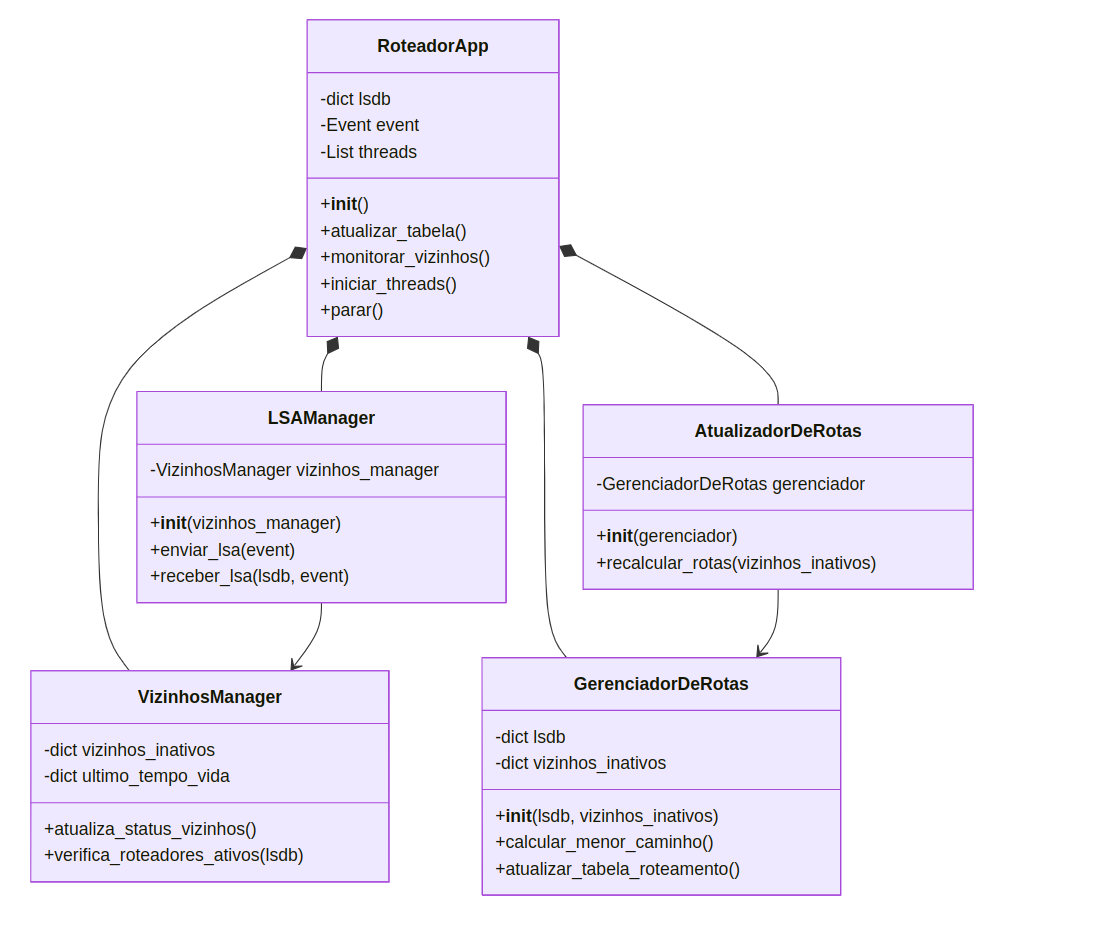
\includegraphics[width=0.8\textwidth]{diagrama_classes.png}
    \caption{Representação da arquitetura}
    \label{fig:classes}
\end{figure}

\chapter{Resultados}
Nesta seção, serão apresentados os resultados obtidos durante a fase de testes, bem como a análise das questões propostas pelo professor. As reflexões abordarão os seguintes pontos: quais são os limites e o nível de estresse suportado pelo sistema; quais as principais vantagens da abordagem adotada; se é possível que um \textit{host} realize um \textit{ping} com sucesso para outro \textit{host}; e, por fim, qual foi a estratégia de implementação utilizada e os motivos que justificam essa escolha.

\section{Limiares/Stress}
Para responder a essa pergunta, optei por analisar duas métricas fundamentais: tempo e taxa de acerto. Essas métricas refletem diretamente os objetivos centrais em redes de computadores — alcançar comunicações cada vez mais rápidas e eficientes. O tempo representa a agilidade do sistema em propagar informações e estabelecer rotas, enquanto a taxa de acerto avalia a precisão das decisões de roteamento, indicando se os pacotes estão sendo encaminhados corretamente ao destino final.

\subsection{Tempo de Resposta Entre Roteadores}
\begin{figure}[h!]
    \centering
    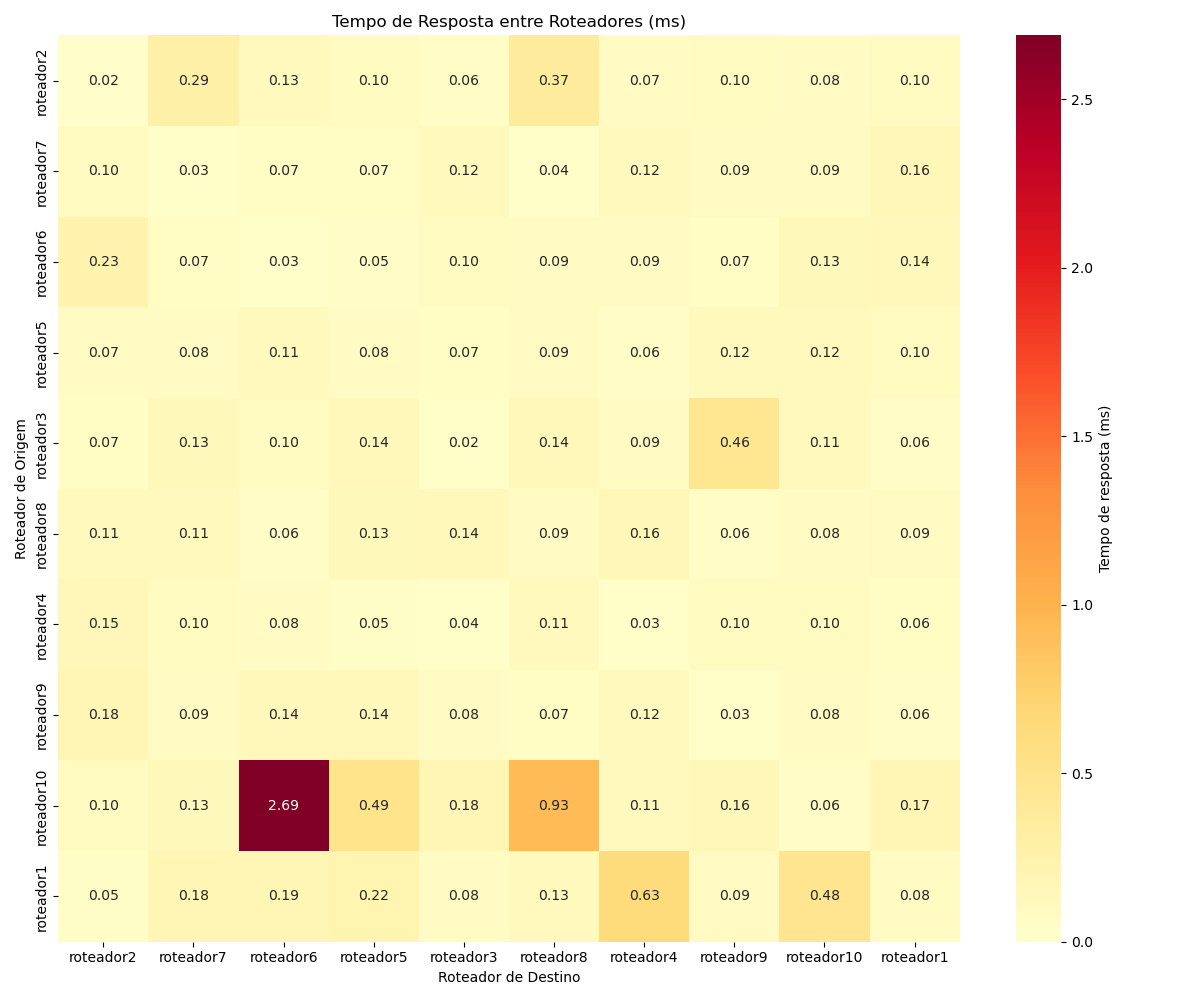
\includegraphics[width=0.6\textwidth]{matriz_tempos_resposta.png}
    \caption{Tempo de Resposta Entre Roteadores}
    \label{fig:matriz}
\end{figure}

A Figura \ref{fig:matriz} apresentada é um mapa de calor que representa o tempo de resposta entre pares de roteadores em milissegundos (ms). Cada célula indica o tempo médio de comunicação entre um roteador de origem (eixo vertical) e um roteador de destino (eixo horizontal). Em geral, os tempos de resposta são baixos, variando predominantemente entre 0.02 ms e 0.20 ms, o que demonstra um desempenho eficiente na maioria das comunicações. No entanto, há um ponto de destaque em vermelho entre o \textit{roteador5} e o \textit{roteador8}, com um tempo significativamente mais alto (0.63 ms), sugerindo um gargalo ou instabilidade momentânea naquela conexão.

Outro aspecto relevante a ser analisado diz respeito aos valores presentes na diagonal principal da matriz de tempos de resposta, os quais representam o \textit{ping} realizado pelos roteadores para si mesmos. Esses tempos são significativamente menores em comparação com os tempos de comunicação entre diferentes roteadores, o que é esperado, uma vez que não envolvem tráfego real na rede física. Esse comportamento confirma que o sistema está operando corretamente, já que as respostas locais ocorrem com latência mínima, refletindo a eficiência interna de processamento e encaminhamento. Além disso, essa observação serve como uma referência importante para avaliar o desempenho relativo das demais comunicações na rede.

\subsection{Taxa de Acertividade entre os Roteadores}
\begin{figure}[h!]
    \centering
    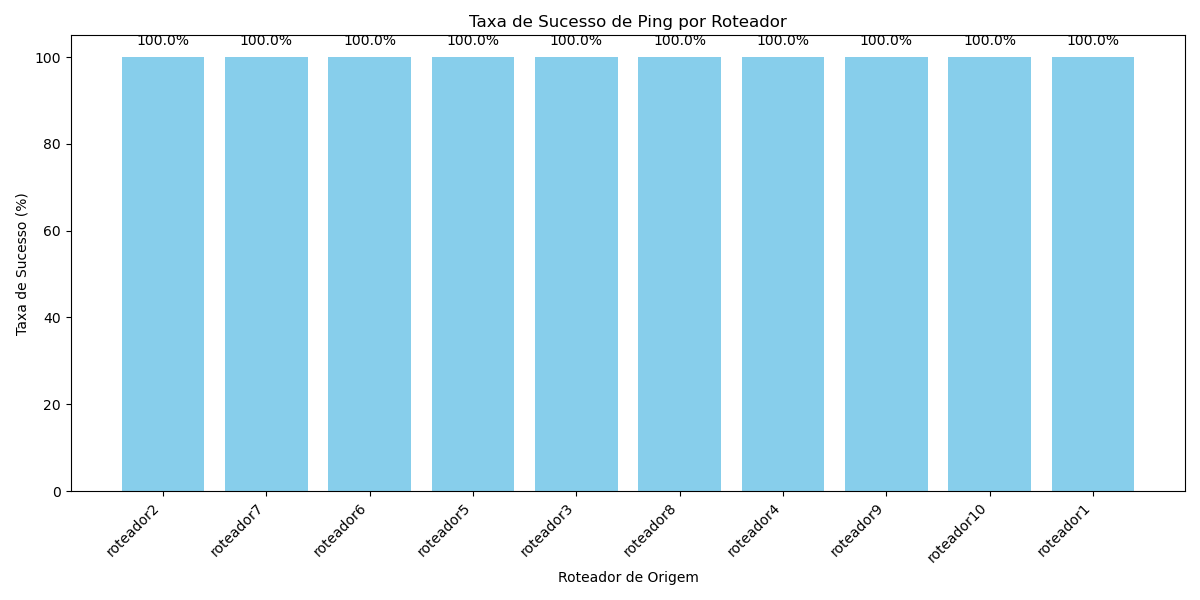
\includegraphics[width=0.6\textwidth]{grafico_taxa_sucesso.png}
    \caption{Taxa de Acertividade entre os Roteadores}
    \label{fig:barras}
\end{figure}

O gráfico apresentado mostra a taxa de sucesso dos testes de \textit{ping} realizados por cada roteador da rede, evidenciando que todos os roteadores atingiram 100\% de sucesso. Esse resultado indica que não houve perda de pacotes durante a comunicação entre os nós, o que reforça a confiabilidade e estabilidade da rede implementada. Além disso, demonstra que o algoritmo de roteamento está operando corretamente, garantindo a entrega eficiente das mensagens entre os dispositivos conectados.

\section{Vantagens e Desvantagens}
\begin{table}[h!]
\centering
\caption{Vantagens e Desvantagens do Sistema}
\begin{tabular}{|p{7cm}|p{7cm}|}
\hline
\textbf{Vantagens} & \textbf{Desvantagens} \\
\hline
\textbf{Eficiência:} O algoritmo de Dijkstra utilizado para calcular as rotas é eficiente e garante a escolha do caminho mais curto. 
& 
\textbf{Complexidade:} A implementação do algoritmo de Dijkstra e o gerenciamento de vizinhos podem aumentar a complexidade do sistema. \\
\hline
\textbf{Robustez:} O sistema é capaz de lidar com falhas de roteadores e \textit{hosts}, garantindo a continuidade do serviço.
&
\textbf{Atualização de Rotas:} A atualização constante das rotas pode gerar um \textit{overhead} significativo, especialmente em redes com alta mobilidade. \\
\hline
\textbf{Atualização Dinâmica:} O sistema é capaz de atualizar suas rotas dinamicamente, adaptando-se a mudanças na topologia da rede.
&
\textbf{Limitações de Escalabilidade:} Embora o sistema seja escalável, a adição de muitos roteadores e \textit{hosts} pode levar a um aumento significativo na complexidade e no tempo de processamento. \\
\hline
\end{tabular}
\end{table}

\section{\textit{Ping} entre \textit{Hosts}}

Para verificar a conectividade fim a fim na rede, foi desenvolvido um \textit{script} de teste específico, que realiza \textit{pings} entre os \textit{hosts} conectados aos roteadores. Esse teste é executado por meio do seguinte comando:

\begin{lstlisting}[language=bash]
make ping_host
\end{lstlisting}

Esse comando automatiza o envio de requisições ICMP entre os \textit{hosts}, permitindo avaliar a comunicação direta através da infraestrutura de roteadores. A seguir, apresenta-se a saída gerada pela execução do script.

\subsection{Saída do Comando \textit{Ping Host}}

\begin{figure}[h!]
    \centering
    \includegraphics[width=0.6\textwidth]{ping.png}
    \caption{Resultado do teste de \textit{ping} entre os \textit{hosts} conectados à rede}
    \label{fig:ping}
\end{figure}

A Figura~\ref{fig:ping} demonstra que os pacotes foram transmitidos com sucesso entre os diferentes \textit{hosts} da rede, evidenciando o correto funcionamento do algoritmo de roteamento e a estabilidade da topologia implementada.

\section{Protocolo de Comunicação Utilizado}

O protocolo adotado para a comunicação entre os \textit{hosts} e os roteadores foi o UDP (\textit{User Datagram Protocol}). Trata-se de um protocolo de transporte leve, que permite a troca de datagramas entre dispositivos de forma rápida e eficiente. Ao contrário do TCP (\textit{Transmission Control Protocol}), o UDP não estabelece uma conexão previamente nem garante a entrega dos pacotes, o que o torna menos confiável, porém substancialmente mais ágil.

Esse protocolo é amplamente empregado em aplicações sensíveis à latência, como transmissões de áudio e vídeo em tempo real, jogos online e sistemas de controle em tempo real, justamente por evitar a sobrecarga de verificação de entrega e controle de fluxo presentes no TCP.

\subsection*{Justificativa para o Uso do UDP}

A escolha do UDP neste projeto fundamenta-se na necessidade de comunicação de baixa latência entre os roteadores e \textit{hosts}. Em um ambiente de simulação de rede, como o aqui proposto, a agilidade na transmissão de mensagens é essencial para representar com fidelidade o comportamento dinâmico da topologia. O UDP proporciona exatamente essa característica, ao permitir o envio assíncrono de pacotes com o mínimo de sobrecarga. Além disso, sua simplicidade de implementação e configuração o torna especialmente adequado para o escopo deste projeto, onde o foco está na eficiência e no desempenho do sistema, e não na confiabilidade absoluta da entrega de pacotes.

\bibliographystyle{sbc}
\bibliography{sbc-template}
\end{document}
